\chapter{Dicom-Presenter}
\vspace{-10mm}
My predecessor Bc. Pavel Neskudla started development of an application for viewing images captured on Magnetic Resonance Imaging (MRI) unit in his Master's thesis\cite{neskudla}. It was a task given by IKEM institute in Prague\footnote{Institute for Clinical and Experimental Medicine}. IKEM institute specialists would utilize some application deployable on personal computers which would offer displaying MRI images. It is possible to find such applications but unfortunately those are too expensive commercial solutions or otherwise freeware applications which do not reach quality requirements\footnote{See \cite[page~9]{flaska_bc} for an overview of accesible DICOM image viewers}. Therefore, IKEM asked FNSPE faculty to develop such an application matching their requirements. Moreover, in this case, the sponsor was allowed to raise unique functionality demands not accessible in other programs (See section \ref{requirements}).

\section{DICOM standard}

DICOM is an abbreviation of Digital Imaging and Communications in Medicine, it is a name of a standard describing medical imaging data manipulation. \footnote{DICOM standard was created by  U.S. National Electrical Manufacturers Association\cite{nema}.} Namely, DICOM standard describes a file format for storing medical data and besides it describes a protocol for exchanging this data. DICOM standard uses common IT standards such as JPEG, TCP/IP, etc.

The main reason why DICOM was created is to avoid medical data confusion. DICOM files are equipped with a header including patient's information. This permanent attachment of header data to DICOM files should avoid random data substitution. There are information about a patient, about medical facility, about a diagnosis in a file header.

\subsection{DICOM viewers}
\label{viewers}
DICOM software is very consumer-specific. Therefore, there are just a few couples of DICOM image viewers available. According to Wikipedia these are the most used DICOM viewers:

\begin{itemize}
  \setlength{\itemsep}{0pt}
  \setlength{\parskip}{0pt}
  \setlength{\parsep}{0pt}
\item \emph{Myrian}, Intrasense, \url{http://www.intrasense.fr/}
\item \emph{NovaPACS}, Novarad, \url{http://www.novapacs.com/}
\item \emph{K-Pacs}, Dr. med. Andreas Knopke, \url{http://www.k-pacs.net/}
\item \emph{DICOM Works}, Philippe PUECH, Loïc BOUSSEL, \url{http://dicom.online.fr/}
\item \emph{OsiriX}, OsiriX Foundation, \url{http://www.osirix-viewer.com/}
\item \emph{Aeskulap}, Alexander Pipelka, \url{http://aeskulap.nongnu.org/}
\item \emph{kradview}, David Santo Orcero, \url{http://www.orcero.org/irbis/kradview/}
\item \emph{SureVistaVision\texttrademark DICOM Viewer}, MS Technology, \url{http://www.ms-technology.com/medical-solutions/sure-vista-vision.html}
\item \emph{UniPACS},  \url{http://www.idoimaging.com/}
\item \emph{syngo Imaging}, Siemens, \url{http://www.medical.siemens.com/}
\item \emph{VR-Render}, IRCAD, \url{http://www.ircad.fr/softwares/vr-render/Software.php}
\item \emph{MicroDicom}, Simeon Antonov Stoykov, \url{http://www.microdicom.com/}
\end{itemize}

Unfortunately, Myrian, NovaPACS, syngo Imaging and SureVistaVision\texttrademark are commercial applications. Therefore, they are not suitable for IKEM use. OsiriX is very powerful DICOM viewer but it is available only for Max OS X. The variety of DICOM viewers is therefore very limited.

All mentioned DICOM viewers do have very similar appearance. A program GUI is divided into a viewing area and a control area. The application can display a DICOM image in the viewing area or it can display a multi-planar reconstruction of the image. The control area offers image enhancing operations with the image displayed in the viewing area.

\begin{table}[ht]
	\caption{DICOM viewers.}
	\centering
	\begin{tabular}{cc}
			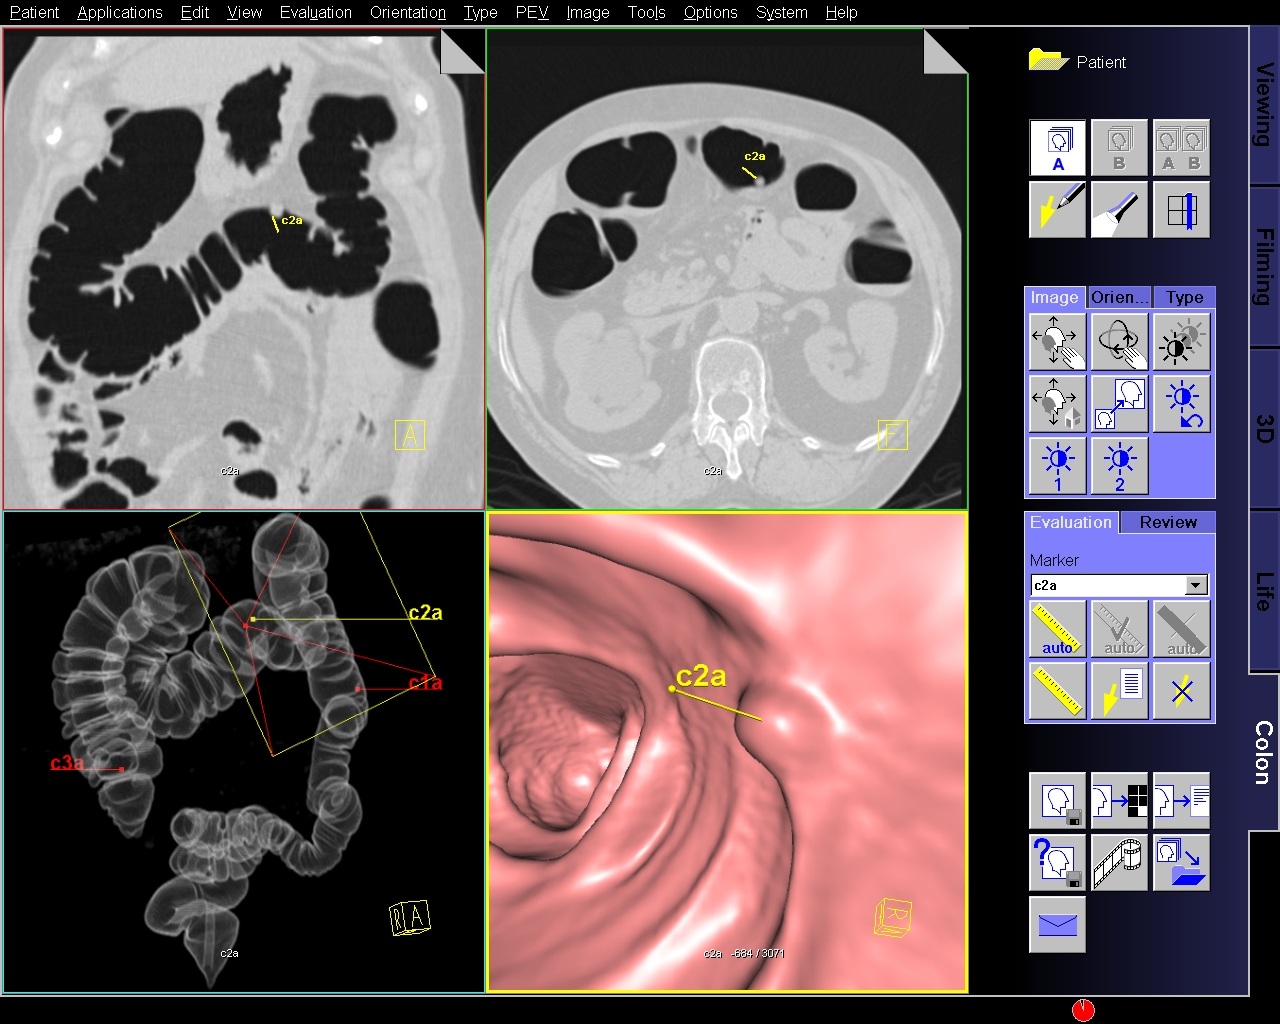
\includegraphics[width=0.5\textwidth,height=0.375\textwidth]{Text/IMG/01_Siemens.jpg}
		&
			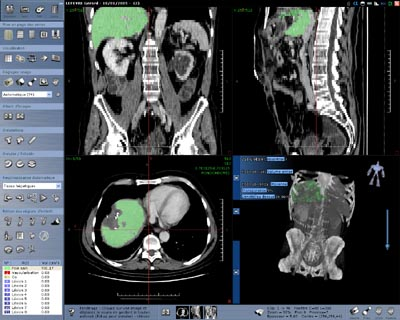
\includegraphics[width=0.5\textwidth,height=0.375\textwidth]{Text/IMG/01_Myrian.jpg}
		\\
			syngo Imaging~\citesec{siemens} & Myrian~\citesec{intrasense}	
		\\
			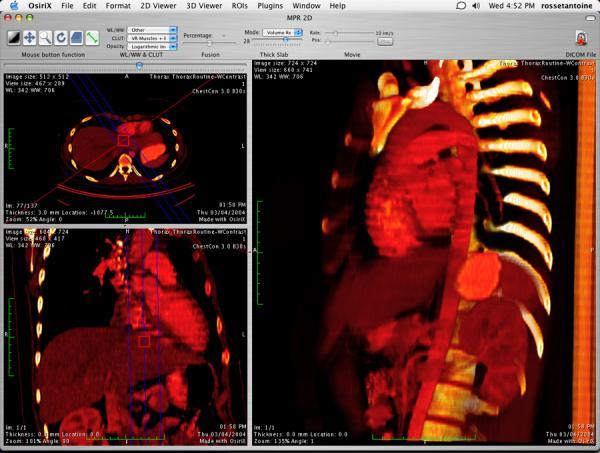
\includegraphics[width=0.5\textwidth,height=0.375\textwidth]{Text/IMG/01_OsiriX.jpg}
		&
			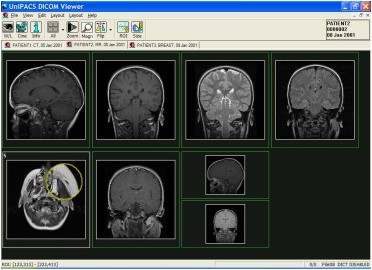
\includegraphics[width=0.5\textwidth,height=0.375\textwidth]{Text/IMG/01_UniPACS.jpg}
		\\
			OsiriX~\citesec{osirix} & UniPACS~\citesec{unipacs}
		\\
		\end{tabular}
\end{table}%




\section{Application Requirements}
\label{requirements}
The IKEM specialists asked for a typical DICOM images viewer with few more specific features which they missed in freeware programs. A typical DICOM viewer allows you to open .dcm files and display it. .dcm file in this case is a jpeg image equipped with special header including patient's information. There you can see a 2D picture of some part of the patient's body. DICOM viewers usually offer opening a set of .dcm files, which can actually fit into a three-dimensional picture. Less commonly it can form a time animation of organ behavior in a short time period (e.g. one heart beat). Some DICOM users offer a multi-planar reconstruction of a picture. Other offered functions may vary.

There have been two specific requirements on application functionality by IKEM specialists. These were not available in freeware DICOM applications. The most important function was the possibility to open several images at once and display them on one screen. The user should be allowed to arrange images on screen to any possible layout he prefers. This functionality allows physicians to see two or more different MRI images on screen so they can easily determine pathological differences among observed organs. It is useful for studying, or teaching.

There have been also requirements that the application should be able to record user's manipulation with images as a video. Then physician can prepare his presentation of images at home and then play the video to colleagues.

\section{Implementation}
After summarizing all the application requirements given by IKEM it was needed to choose proper technologies for application implementation. The aim was to develop a GUI application capable to open and display images, there are several ways to go, so it was the place for a discussion. 

The main question is which programming language to choose. C\#, Java, C++ are the most popular programming languages for extensive GUI applications. C++ offers low level features and thus it offers very good performance. Java and C\# are both interpreted languages. Both were designed to be simple and robust. Altough C\# and Java provide performance simillar to C++ in overall tasks, still C++ reaches better performance in tasks related to imaging. Therefore, C++ was chosen as a programming language of Dicom-Presenter.

A Graphic User Interface of a C++ application is generally written with use of some library. It is possible to write a C++ GUI interface without external library using only OS related function calls but unfortunately this solution brings too complicated source code\footnote{A comparison of GUI interface written with and without external library can be found in Section \ref{noqt}}. There are more then ten application frameworks possible to be used for writing C++ GUI application. Qt and GTK are the most popular libraries used in many commercial applications and offering extensive possibilities for C++ application programming\cite{wikipedia}. Besides GUI creation Qt and GTK offers assistance with image manipulation, network access, xml parsing, etc. Both libraries are cross-platform. Finally, Qt was used to better documentation offered by its author.

There was a research idea when creating Dicom-Presenter: check possibility of using GPU in this kind of application. Dicom-Presenter will have to handle with large graphic data. If GPU and its memory will handle this data a great performance enhancement could be reached. Therefore, OpenGL library was used for all image manipulation in Dicom-Presenter. It solves image storing, image manipulations and image rendering. Unfortunately, OpenGL brings 
occasional uncompatibility on some hardware which was unacceptable so the main goal of this project is to remove OpenGL from Dicom-Presenter. If OpenGL library would be replaced then also dependencies on Cg toolkit library and plib library would be removed it would highly simplify project compilation and enhance compatibility.



\section{Functionality}
\label{dicom-presenter}
Dicom-Presenter design is based on appearance of other DICOM image viewers. The goal was to display images and perform basic image manipulation. The application window can be divided into two main parts: a rendering part and control part. Rendering part itself is divided into three sub-parts. Most of the place is naturally reserved for image rendering (later called Workspace). Bottom part is used for switching workspaces (later called Workspace Explorer). A side part or rendering window is used for accessing images stored in application memory (later called Image Explorer). Next to the rendering part is a control window which allows user to watch image  properties and adjust them numerically (later called Control Panel). 

Above described concept is very similar to appearance of other viewers unlike the part allowing workspace switching. It is a feature required by IKEM not supported in any of DICOM viewers mentioned in \ref{viewers}.

The basic scenario of Dicom-Presenter work session can be described in the following way: After running the application user clicks ``Open Dicom Image'' button located on the control panel. Then the image preview appears in the Image Explorer. By clicking the image preview the image becomes a Selected Object. There is only one Selected Object in Dicom-Presenter at the time. A key property of the Selected Object is that the Control Panel contains its information. Therefore, after declaring the opened image as selected a button called ``Create Image Copy'' appears in the Control Panel. By clicking the mentioned button the image appears on the Workspace. If we need to open one more image we click the proper button again. Afterwards a second image preview appears in Image Explorer. Then the necessity of Image Explorer becomes clear.

User is allowed to freely customize the image arrangement on the Workspace. This is a notable feature in Dicom-Presenter. None of the DICOM viewers mentioned in \ref{viewers} offers it. Therefore, it was a request from IKEM that image layout has to be fully customizable. Images can be easily moved  by clicking any image at a proper place and dragging it on the Workspace.  It is a user-friendly powerful feature.

As was said before, Dicom-Presenter is aimed to allow presenting images to other physicians. To avoid a need of picture manipulation during a presentation, a possibility of having more workspaces opened was implemented. Each workspace can be prepared before presenting and stored in application memory.
 
\begin{figure}
	\begin{center}
	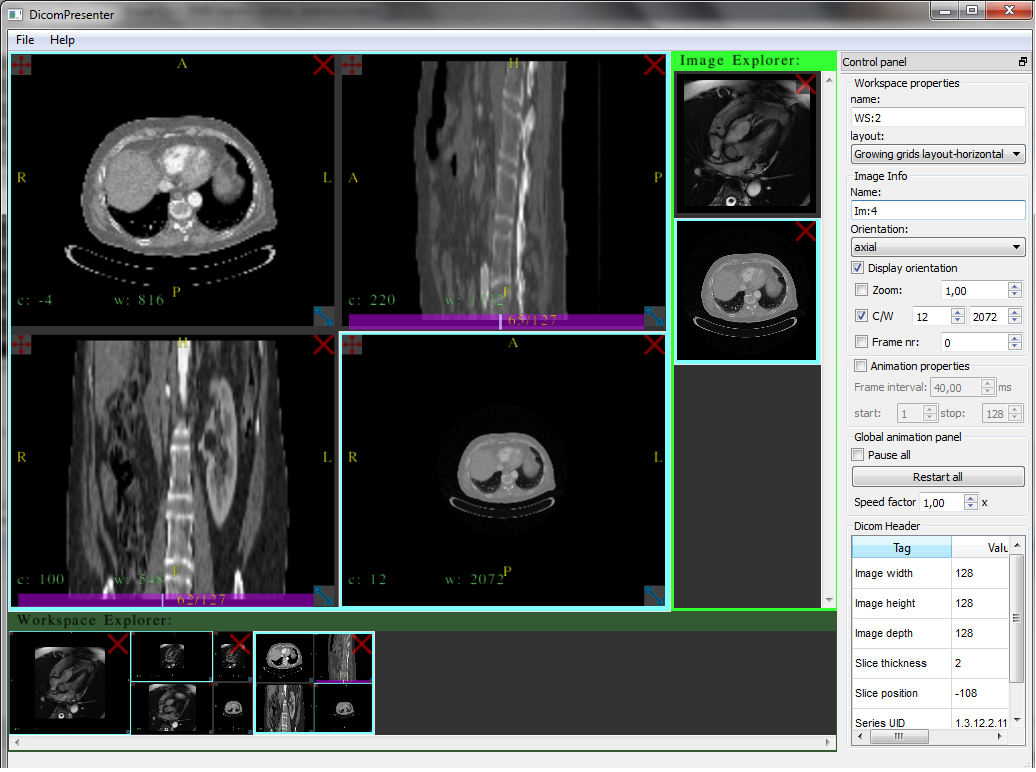
\includegraphics[width=130mm]{Text/IMG/04_GUI_Screenshot.png}
	\end{center}
	\caption{Screenshot of Dicom-Presenter user interface.}
	\label{screenshot}
\end{figure}